\documentclass[12pt]{article}
%\usepackage[utf8]{inputenc}
%\documentclass[UTF8]{ctexart}
%\usepackage[UTF8, heading = false, scheme = plain]{ctex}
\usepackage{geometry}
%geometry{a4paper,scale=0.9}
\geometry{a4paper,left=1cm,right=1cm,top=1cm,bottom=2cm}
\usepackage{amsfonts}
\usepackage{color}
\usepackage{url}
%\usepackage{biblatex}
\usepackage{amsmath}
\usepackage{amssymb}
\usepackage{latexsym}
\usepackage{cite}
%\addbibresource{ref.bib}
%\bibliography{ref.bib}
\usepackage{caption}
\usepackage{graphicx, subfig}
\usepackage{float}
%\usepackage[fontset=ubuntu]{ctex}
%\usepackage{fontspec}
\usepackage{xeCJK}
%\usepackage[colorlinks,
%anchorcolor=black,
%citecolor=black]{hyperref}
%\setmainfont{SimSun}
\usepackage[section]{placeins}
\usepackage{enumitem}
\usepackage{framed}
\usepackage[framemethod=TikZ]{mdframed}
\usepackage{indentfirst}
\usepackage{setspace}%使用间距宏包
\linespread{1.5}
%\title{预备知识}
%\author{leolinuxer }
%\date{June 2020}

\title{凸优化\cite{Understand_Convex_Optimization_In_One_Article}}
%\author{leolinuxer }
%\date{June 2020}

\begin{document}
\maketitle

\section{几何体的向量表示}
在介绍凸集等概念之前,首先介绍一下空间几何体的向量表示,下面在定义凸集概念时便用到了线段的线段表示。先通过一个例子来认识一下如何使用向量表示线段。

已知二维平面上两定点$A(5, 1)$、$B(2,3)$,给出线段$AB$的方程表示如下:
$$
\begin{cases}
x_1 = \theta \times 5 + (1 - \theta) \times 2 \\
x_2 = \theta \times 1 + (1 - \theta) \times 3 \\
\end{cases}
\quad \theta \in [0, 1]
$$

如果将点$A$看成向量$\vec{a}$,点$B$看成向量$\vec{b}$,则线段$AB$的向量表示为:
$$
\vec{x} = \theta \vec{a} + (1-\theta) \vec{b}, \quad \theta \in [0,1]
$$

而直线的向量表示是:
$$
\vec{x} = \theta \vec{a} + (1-\theta) \vec{b}, \quad \theta \in \mathbb{R}
$$

由此衍生推广到高维,可得以下几何体的向量表示,三角形的向量表示:
$$
\vec{x} = \theta_1 \vec{a_1} + \theta_2 \vec{a_2} + \theta_3 \vec{a_3}, \quad \theta_i \in [0,1], \sum\theta_i = 1
$$

三维平面的向量表示:
$$
\vec{x} = \theta_1 \vec{a_1} + \theta_2 \vec{a_2} + \theta_3 \vec{a_3}, \quad \theta_i \in \mathbb{R}, \sum\theta_i = 1
$$

超几何体的向量表示:
$$
\vec{x} = \theta_1 \vec{a_1} + \theta_2 \vec{a_2} + \cdots + \theta_k \vec{a_k}, \quad \theta_i \in [0,1], \sum\theta_i = 1
$$

超平面的向量表示:
$$
\vec{x} = \theta_1 \vec{a_1} + \theta_2 \vec{a_2} + \cdots +  \theta_k \vec{a_k}, \quad \theta_i \in \mathbb{R}, \sum\theta_i = 1
$$

\section{凸集凸函数定义}
\subsection{凸集}
集合$C$内任意两点间的线段也均在集合$C$内,则称集合$C$为凸集,数学定义为:
$$
\forall x_1,x_2 \in C, \forall \theta \in [0,1], \text{则} x = \theta\cdot x_1 + (1-\theta)\cdot x_2 \in C
$$

$k$个点的版本:
$$
\forall x_1, x_2, \cdots x_k \in C, \theta_i \in [0,1], \text{且} \sum\theta_i = 1, \text{则} x = \sum_{i=1}^k\theta_ix_i \in C
$$

上面凸集定义中便用到了线段的向量表示,含义是如果点$x_1$和点$x_2$在集合$C$内,则线段$x_1x_2$上所有点都在集合$C$内,凸集的交集仍是凸集。

\subsection{凸函数}
\textbf{凸函数}定义为,设$f \subseteq \mathbb{R}^n \to \mathbb{R}^1$,$C$是凸集,对于$x_1, x_2 \in C$ 都有:
$$
f(\alpha_1x_1 + \alpha_2x_2) \le \alpha_1f(x_1) + \alpha_2f(x_2) \quad \sum\alpha_i = 1, \alpha_i \ge 0
$$

则称 $f(x)$ 为定义在凸集$C$上的凸函数。

\textbf{严格凸函数}定义为,设$f \subseteq \mathbb{R}^n \to \mathbb{R}^1$,$C$是凸集,对于$x_1, x_2 \in C$ 都有:
$$
f(\alpha_1x_1 + \alpha_2x_2) < \alpha_1f(x_1) + \alpha_2f(x_2) \quad \sum\alpha_i = 1, \alpha_i \ge 0
$$

则称 $f(x)$ 为定义在凸集$C$上的严格凸函数。

凸函数的等价定义:设$f \subseteq \mathbb{R}^n \to \mathbb{R}^1$,$C$是凸集,对于$x_1, x_2, x_3 \in C $且$x_1<x_2<x_3$,下式成立则 $f(x)$为凸函数(??待证明??):
$$
\frac{f(x_2) - f(x_1)}{x_2 - x_1} \le \frac{f(x_3) - f(x_1)}{x_3 - x_1} \le \frac{f(x_3) - f(x_2)}{x_3 - x_2}
$$

\section{凸函数各种性质及其证明}
\subsection{性质-下水平集}
设 $f \subseteq \mathbb{R}^n \to \mathbb{R}^1$,$C$是凸集,若$f$是凸函数,则对于$\forall\beta$,证明下面水平集$D_\beta$是凸集
$$
D_\beta = \{x|f(x) \le \beta, x \in C\}
$$
\begin{framed}  
%\verb|\documentstyle[ifthen,12pt,titlepage]{article}|
\small{
证明:若对于 $\forall x_1,x_2 \in D_beta$,则线段 $x_1x_2$为:
$$
    x_1x_2 = \alpha_1x_1 + \alpha_2x_2, \alpha_i > 0, \sum\alpha_i = 1
$$
且因为 $f(x)$ 是凸函数,所以:
$$
f(\alpha_1x_1 + \alpha_2x_2) \le \alpha_1f(x_1) + \alpha_2f(x_2) \le \alpha_1\beta + \alpha_2\beta = \beta
$$

所以原命题得证,水平集 $D_\beta$ 是凸集。
}
\end{framed}

\subsection{性质-全局最优}
凸优化问题的局部极小值是全局极小值。

这个性质是凸优化问题一个良好的性质,在机器学习任务中我们只需将非凸问题转化为凸优化问题,便可直接求出问题的全局极值,下面给出证明:
\begin{framed}  
%\verb|\documentstyle[ifthen,12pt,titlepage]{article}|
\small{
反证法证明:假定 $x^*$ 是局部极小点,不是全局极小点,则一定存在 $x'$ 使得:
$$
f(x') < f(x^*)
$$

构造凸组合点 $x = \alpha_1x' + \alpha_2x^*, \quad \sum\alpha_i = 1$,有:
$$
f(x) = f(\alpha_1x' + \alpha_2x^*) \le \alpha_1f(x') + \alpha_2f(x^*) < \alpha_1(f^*) + \alpha_2f(x^*) = f(x^*)
$$

当 $\alpha_2 \to 1$时,$x$点无限趋近于 $x^*$,即 $x$ 是 $x^*$ 邻域中的一点,但仍然存在 $f(x) < f(x^*)$,与 $x^*$是局部极小点矛盾;因此原问题得证。
}
\end{framed}

\subsection{性质-梯度}
设 $f \subseteq \mathbb{R}^n \to  \mathbb{R}^1$,$C$是凸集,对于$x_1, x_2 \in C$,

(1) $f$为凸函数的充要条件是:对于$\forall x_1, x_2 \in C$且$x_1 \neq x_2$都有:
$$
f(x_2) \ge f(x_1) + \nabla f(x_1)^T(x_2-x_1)
$$

(2) f为严格凸函数的充要条件是:对于$\forall x_1, x_2 \in C$且$x_1 \neq x_2$都有:
$$
f(x_2) > f(x_1) + \nabla f(x_1)^T(x_2-x_1)
$$

\begin{framed}  
%\verb|\documentstyle[ifthen,12pt,titlepage]{article}|
\small{
证明:先证明充分性,即 $f(x)$ 是凸函数 $\Rightarrow$ $f(x_2) \ge f(x_1) + \nabla f(x_1)^T(x_2-x_1)$

因为 $f(x)$ 是凸函数,所以 $\alpha_1, \alpha_2 \in [0,1], \sum\alpha_i = 1$,有:
$$
f(\alpha_1x_1 + \alpha_2x_2) \le \alpha_1f(x_1) + \alpha_2f(x_2)
$$

令 $\alpha_1 = 1 - t, \alpha_2 = t$,有:
$$
f((1-t)x_1 + tx_2) \le (1-t)f(x_1) + tf(x_2)
$$
$$
f(x_1 + t(x_2-x_1)) \le f(x_1) + t(f(x_2) - f(x_1))
$$
$$
\frac{f(x_1 + t(x_2-x_1)) - f(x_1)}{t} \le f(x_2) - f(x_1)
$$

用极限的思想:

$$\lim_{t \to 0}\frac{f(x_1 + t(x_2-x_1)) - f(x_1)}{t} = \nabla f(x_1)^T(x_2 - x_1)$$

所以:
$$
\nabla f(x_1)^T(x_2 - x_1) \le f(x_2) - f(x_1)
$$
故充分性得证;

再证明必要性,即$f(x_2) \ge f(x_1) + \nabla f(x_1)^T(x_2-x_1)$ $\Rightarrow$  $f(x)$ 是凸函数

$\forall x_1, x_2 \in C$,有$x = \alpha_1x_1 + \alpha_2x_2$,其中$\alpha_1, \alpha_2 \in [0,1], \sum\alpha_i = 1$,所以:
$$
f(x_1) \ge f(x) + \nabla f(x)^T(x_1-x) 
$$
$$
f(x_2) \ge f(x) + \nabla f(x)^T(x_2-x) 
$$

所以:
$$
\alpha_1f(x_1) \ge \alpha_1f(x) + \nabla f(x)^T\alpha_1(x_1-x) 
$$
$$
\alpha_2f(x_2) \ge \alpha_2f(x) + \nabla f(x)^T\alpha_2(x_2-x) 
$$
$$
\alpha_1f(x_1) + \alpha_2f(x_2) \ge (\alpha_1+\alpha_2)f(x) + \nabla f(x)^T(\alpha_1x_1 + \alpha_2x_2 - (\alpha_1+\alpha_2)x)
$$

因为 $\alpha_1 + \alpha_2 = 1$,所以有:
$$
\alpha_1f(x_1) + \alpha_2f(x_2) \ge f(x) = f(\alpha_1x_1 + \alpha_2x_2)
$$
故必要性得证。
}
\end{framed}

\subsection{性质-Hessian矩阵}
凸函数的Hessian矩阵半正定。

该性质描述了凸函数二阶可微时满足的性质,即凸函数的Hessian矩阵半正定,此性质可通过泰勒公式进行,在给出该性质证明之前,先给出Hessian矩阵和泰勒公式定义。

Hessian矩阵是一个多元函数的二阶偏导数构成的方阵,一个多元函数Hessian矩阵定义如下:
$$
H(f) = J(J(f)) =
\begin{bmatrix}
\frac{\partial^2 f}{\partial x_1^2} & \frac{\partial^2 f}{\partial x_2\partial x_1} & \cdots & \frac{\partial^2 f}{\partial x_n\partial x_1}  \\
\frac{\partial^2 f}{\partial x_1\partial x_2} & \frac{\partial^2 f}{\partial x_2^2} & \cdots & \frac{\partial^2 f}{\partial x_n\partial x_2}  \\
\vdots & \vdots &  & \vdots \\
\frac{\partial^2 f}{\partial x_1\partial x_n} & \frac{\partial^2 f}{\partial x_2\partial x_n} & \cdots & \frac{\partial^2 f}{\partial x_n^2}  \\
\end{bmatrix}
$$

一般情况下,多元函数的混合二阶偏导数与求导次序无关\cite{Understand_Convex_Optimization},即:
$$
\frac{\partial^2 f}{\partial x_i\partial x_j} = \frac{\partial^2 f}{\partial x_j\partial x_i}
$$

因此Hessian矩阵是一个对称矩阵,它可以看作二阶导数对多元函数的推广。Hessian矩阵简写为$\nabla^2 f(x)$ 。对于如下多元函数:
$$
f(x,y,z) = 2x^2 - xy + y^2 - 3z^2
$$

它的Hessian矩阵为:
$$
\begin{bmatrix}
\frac{\partial ^2f}{\partial x^2} & \frac{\partial ^2f}{\partial x \partial y} & \frac{\partial ^2f}{\partial x \partial z} \\
\frac{\partial ^2f}{\partial y \partial x} & \frac{\partial ^2f}{\partial y^2} & \frac{\partial ^2f}{\partial y \partial z} \\
\frac{\partial ^2f}{\partial z \partial x} & \frac{\partial ^2f}{\partial z \partial y} & \frac{\partial ^2f}{\partial z^2} \\
\end{bmatrix} = 
\begin{bmatrix}
4 & -1 & 0\\ -1 & 2 & 0\\ 0 & 0 & -6\\
\end{bmatrix}
$$

根据多元函数极值判别法,假设多元函数在点M的梯度为0,即M是函数的驻点,则有:
\begin{itemize}
\setlength{\itemsep}{0pt}
\setlength{\parsep}{0pt}
\setlength{\parskip}{0pt}
    \item 如果Hessian矩阵正定,函数在该点有极小值
    \item 如果Hessian矩阵负定,函数在该点有极大值
    \item 如果Hessian矩阵不定,则不是极值点(鞍点)
\end{itemize}

这可以看做是一元函数极值判别法对多元函数对推广,Hessian矩阵正定类似于二阶导数大于0,其他的以此类推。对于$n$阶矩阵$A$,对于任意非0的$n$维向量$x$都有:
$$
x^TAx > 0
$$

则称矩阵A为正定矩阵。判定矩阵正定的常用方法有以下几种:
\begin{itemize}
\setlength{\itemsep}{0pt}
\setlength{\parsep}{0pt}
\setlength{\parskip}{0pt}
    \item 矩阵的特征值全大于0;
    \item 矩阵的所有顺序主子式都大于0;
    \item 矩阵合同于单位阵I;
\end{itemize}

泰勒公式是用若干项连加来表示一个函数,这些相加的项由函数在某一点的导数求得,下面给出一个函数$f(x)$在$x=a$点的泰勒展开式:
$$
f(x) = \frac{f(a)}{0!} + \frac{f'(a)}{1!}(x-a) + \frac{f''(a)}{2!}(x-a)^2 + \cdots + \frac{f^{(n)}(a)}{n!}(x-a)^n + R_n(x)
$$

\begin{framed}  
%\verb|\documentstyle[ifthen,12pt,titlepage]{article}|
\small{
证明:
Hessian 矩阵可看做:$\nabla^2f(x)$

对于凸函数$f(x)$,有$f(x) \ge f(x_0) + \nabla f(x_0)^T(x-x_0)$,

将 $f(x)$ 进行泰勒展开,有
$$
f(x) = f(x_0) + \nabla f(x_0)^T(x-x_0) + \frac{1}{2}(x-x_0)^T\nabla^2f(x_0)^T(x-x_0) + R(n)
$$

其中 $R(n)$ 是余项,关于 $(x-x_0)^2$ 的高阶无穷小,即$R(n) \to 0$

因此:
$$
\frac{1}{2}(x-x_0)^T\nabla^2f(x_0)^T(x-x_0) \ge 0
$$

其中 $x-x_0 \in \mathbb{R}^n, H(f) = \nabla^2f(x_0)^T$,所以:
$$
(x-x_0)^T\nabla^2f(x_0)^T(x-x_0) \ge 0
$$

因此$H$ 半正定,问题得证。
}
\end{framed}

\subsection{性质}
若 $x \in \mathbb{R}^n, y \in \mathbb{R}^n$(即 $x,y$为$n$维空间向量),$Q$为半正定对称阵,则 $f(x) = X^TQX$为凸函数
\begin{framed}  
%\verb|\documentstyle[ifthen,12pt,titlepage]{article}|
\small{
证明:要证明 $f(x) = X^TQX$为凸函数,需要证明:
$$
f(\alpha x + (1-\alpha)y) \le \alpha f(x) + (1-\alpha)f(y)
$$
其中,$x\in \mathbb{R}^n, y\in \mathbb{R}^n, \alpha \in [0,1]$

令
\begin{align*}
F &= f(\alpha x + (1-\alpha)y) - \alpha f(x) - (1-\alpha)f(y)  \\
  &= (\alpha x + (1-\alpha)y)^TQ(\alpha x + (1-\alpha)y) - \alpha x^TQx - (1-\alpha)y^TQy \\
  &= \alpha^2x^TQx + (1-\alpha)^2y^TQy + \alpha(1-\alpha)x^TQY + \alpha(1-\alpha)y^TQx - \alpha x^TQx - (1-\alpha)y^TQy
\end{align*}

因为 $Q$ 是对称阵,即 $Q^T = Q$,所以:
$$
x^TQy = (y^TQ^Tx)^T = (y^TQx)^T = y^TQ^Tx 
$$
最后一步等号是因为$(y^TQx)^T \in \mathbb{R}^1$,所以 $(y^TQx)^T = y^TQ^Tx$


所以:
$$
F = \alpha(\alpha-1)(x^TQx - 2x^TQy + y^TQy) = \alpha(\alpha-1)(x-y)^TQ(x-y)
$$

因为 $Q$ 是半正定阵,所以对 $(x-y) \in \mathbb{R}^n$,有
$$
(x-y)^TQ(x-y) \ge 0
$$
所以 $F \le 0$,所以 $f(\alpha x + (1-\alpha)y) \le \alpha f(x) + (1-\alpha)f(y)$,即问题得证
}
\end{framed}

\subsection{性质-Jensen不等式前奏}
凸函数$f(x)$,其中$Q_1+Q_2+…+Q_n=1,0<= Q_i<=1$,证明下面不等式:
$$
f(Q_1x_1 + Q_2x_2 + \cdots + Q_nx_n) \le Q_1f(x_1) + Q_2f(x_2) + \cdots + Q_nf(x_n)
$$

\begin{framed}  
%\verb|\documentstyle[ifthen,12pt,titlepage]{article}|
\small{
使用数学归纳法证明:

假设,$n=2$ 时成立,即:$f(Q_1x_1 + Q_2x_2) \le Q_1f(x_1) + Q_2f(x_2)$

假设,$n=k$ 时成立,即:$f(Q_1x_1 + Q_2x_2 + \cdots + Q_kx_k) \le Q_1f(x_1) + Q_2f(x_2) + \cdots + Q_kf(x_k)$


则当 $n=k+1$时,有:
\begin{align*}
F &= Q_1f(x_1) + Q_2f(x_2) + \cdots + Q_kf(x_k) +  Q_{k+1}f(x_{k+1}) \\
  &= (1-Q_{k+1})\frac{1}{(1-Q_{k+1})}(Q_1f(x_1) + Q_2f(x_2) + \cdots + Q_kf(x_k)) + Q_{k+1}f(x_{k+1})
\end{align*}

根据 $n=k$ 时,$\frac{\sum_{i=1}^kQ_i}{1-Q_{k+1}} = 1$, 有
\begin{align*}
    F &\ge (1-Q_{k+1})f(\frac{Q_1f(x_1) + Q_2f(x_2) + \cdots + Q_kf(x_k)}{1-Q_{k+1}}) + Q_{k+1}f(x_{k+1}) \\
  &\ge f(Q_1x_1 + Q_2x_2 + \cdots + Q_kx_k + Q_{k+1}x_{k+1})
\end{align*}

所以命题得证。
}
\end{framed}

\subsection{性质-Jensen不等式}
Jessen不等式,$f(x)$为凸函数,其中$E(x)$是$x$的期望,则:
$$
f(E[x]) \le E[f(x)]
$$

\begin{framed}  
%\verb|\documentstyle[ifthen,12pt,titlepage]{article}|
\small{
根据上述性质,可以快速得证。
}
\end{framed}

Jensen不等式的直观理解:
\begin{figure}[H]
    \centering
    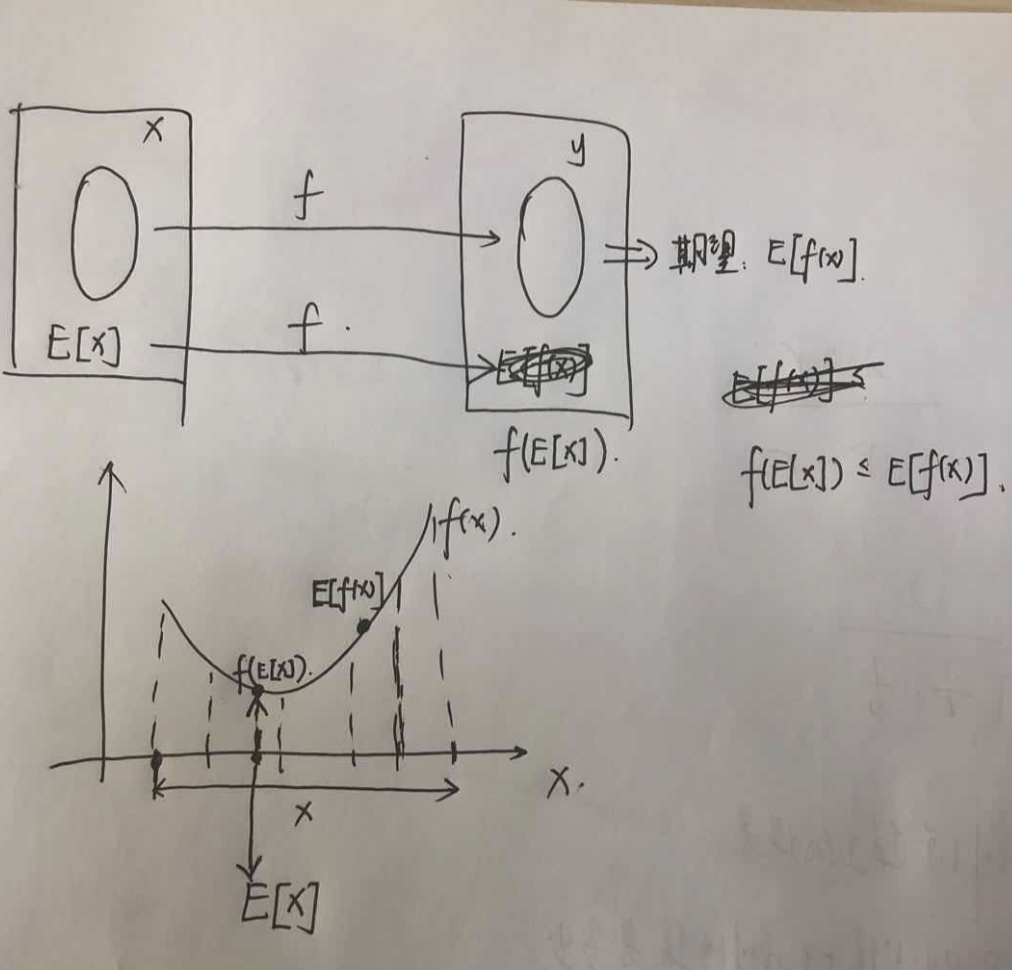
\includegraphics[width=.6\textwidth]{fig/Jensen_Unequal_Example.png}
\end{figure}

\section{凸优化}
\subsection{凸优化问题定义}
一个凸优化问题可描述为:
$$
f(x) \quad s.t. \quad x\in C
$$
$$
s.t. \quad g_i(x) <= 0, h_i(x) = 0
$$

通过以下凸优化性质便可理解何为凸优化问题:

(1) 目的是求解目标函数的最小值;

(2) 目标函数$f(x)$和不等式约束函数$g(x)$都是凸函数,定义域是凸集;

(3) 若存在等式约束函数,则等式约束函数$h(x)$为仿射函数;仿射函数指的是最高次数为1的多项式函数,一般形式为$f(x)= Ax + b$,$A$是$m*k$矩阵,$x$是一个$k$向量,$b$是一个$m$向量

(4) 凸优化问题有一个良好的性质即:局部最优解便是全局最优解

\subsection{常见凸优化问题}
\subsubsection{线性规划LinearProgramming(LP)}
如果目标函数和不等式约束函数都是仿射函数,则凸优化问题称为线性规划,数学表示为:
$$
C^Tx + d
$$
$$
s.t.\quad Gx <= h, Ax = b
$$

\subsubsection{二次规划QuadraticProgramming(QP)}
如果目标函数是凸二次函数,而不等式约束仍是仿射函数,则凸优化问题称为二次规划,数学表示为:
$$
\frac{1}{2}x^TPx + c^Tx + d
$$
$$
s.t.\quad Gx <= h, Ax = b
$$

\subsubsection{ 二次约束的二次规划 Quadratically Constrained Quadratic Programming(QCQP)}
如果目标函数和不等书约束均为凸二次函数,则凸优化问题称为二次约束的二次规划,数学表示为:
$$
\frac{1}{2}x^TPx + c^Tx + d
$$
$$
s.t.\quad \frac{1}{2}x^TQ_ix + r_i^Tx + s_i <= 0, \quad i = 1, 2, \cdots, m, \quad Ax = b
$$

\subsubsection{半正定规划Semidefinite Programming(SDP)}
半正定规划较前面的复杂,在机器学习中也经常用到,下面给出数学描述:
$$
tr(CX)
$$
$$
s.t. \quad tr(A_ix) = b_i \quad i = 1, 2, \cdots, p, \quad X >= 0
$$
其中符号$tr(A)$表示矩阵$A$的迹,矩阵$A$的迹是指$A$的对角线上各个元素的总和

\section{浅谈凸优化问题为何如此重要}
1、凸优化具有良好性质,如局部最优解是全局最优解,且凸优化问题是多项式时间可解问题,如:线性规划问题;

2、很多非凸优化或NP-Hard问题可以转化成凸优化问题,方法:对偶、松弛(扩大可行域,去掉部分约束条件),在SVM算法中,为了对目标函数进行优化,便使用了拉格朗日乘子法、对偶问题、引入松弛因子等。

\bibliography{../ref}
\bibliographystyle{IEEEtran}
\end{document}
